%--------------------------------------------------------------------------------------------------
% OBSERVACAO:
% 
% -> Arquivos que você pode editar:
%    - artigo.tex
%    - artigo_bibliografia.bib
%
% -> Arquivo .TeX codificado em UTF8                                                             
% -> Bibliografia em arquivo .bib (arquivo_bibliografia.bib)                                      
% -> Arquivo de imagens em .jpg, .eps ou .pdf
% -> Para compilar o TeX, execute 'compila_TEX.bat' (terminal do windows)
% 
% versão 1.1 - 19/05/2016
% versão 1.0 - 18/08/2015
%--------------------------------------------------------------------------------------------------
\documentclass{classe_cn}                 % Modelo <nao edite o arquivo classe_cn.cls>
\usepackage[brazil]{babel}                % Acentos
\usepackage[utf8]{inputenc}               % Codificação UTF8 (atenção aqui!)
\usepackage{graphicx}                     % Figura
\usepackage{amssymb}                      % Simbolos matematicos
\usepackage{color}                        % Cores
\usepackage{amsfonts}                     % Fontes
\usepackage{amsmath}                      % Fontes
\usepackage[fixlanguage]{babelbib}        % Acentos
\usepackage[normalem]{ulem}               % OK
\usepackage[retainorgcmds]{IEEEtrantools} % Formulas padrão IEEE
\usepackage{omlmathbf}                    % Simbolos Matematicos
\usepackage{epstopdf}                     % Figuras .eps
\usepackage{setspace}                     % Espaçamento flexível
\usepackage{cmap}                         % Mapear caracteres especiais no PDF
\usepackage{textcomp}                     % Funções e outros símbolos matemáticos
\usepackage{verbatim}                     % Pacotes verbatim
\usepackage{wrapfig}
\usepackage{picins}
\startlocaldefs
\endlocaldefs

%--------------------------------------------------------------------------------------------------
% Inicio do Documento
%--------------------------------------------------------------------------------------------------
\begin{document}
\begin{frontmatter}        % Não alterar
\begin{fmbox}              % Não alterar
\dochead{Gerência da Informação} % Não alterar

%--------------------------------------------------------------------------------------------------
% Titulo do seu Trabalho
%   - pequeno bug (nao funciona cedilha)
%   - editar manualmente o cedilha na classe_cn.cls, linha 1015.
%--------------------------------------------------------------------------------------------------
\title{Software Livre para Empresas}

%------------------------------------------------
% Informações sobre o autor #1
% - Antunes Dantas da Silva
%------------------------------------------------
\author[
  addressref = {aff1},                 % Identifica o autor #1
  email      = {antunes.dantas@ccc.ufcg.edu.br} % email para contato
]
{
  \inits{ADdS}      % Letras iniciais do autor #1
  \fnm{Antunes Dantas}  % Nome do autor #1 (first and middle name)
  \snm{da Silva}   % Ultimo nome do autor #1 (last name)
}
%------------------------------------------------
% Informações sobre o autor #2
% - Gabriel Silva Vinha
%------------------------------------------------
\author[
  addressref = {aff1},                      % Identifica o autor
  email      = {gabriel.vinha@ccc.ufcg.edu.br} % email para contato
]
{
  \inits{GSV}       % Letras iniciais do autor #2
  \fnm{Gabriel Silva}  % Nome do autor #2 (first and middle name)
  \snm{Vinha}    % Ultimo nome do autor #2 (last name)
}
%------------------------------------------------
% Informações sobre o autor #3
% - Italo M. de L. Poroca
%------------------------------------------------
\author[
  addressref = {aff1},                       % Identifica o autor
  email      = {italo.poroca@ccc.ufcg.edu.br} % email para contato
]
{
  \inits{IMdLP}      % Letras iniciais do autor #3
  \fnm{Italo M. de Lima} % Nome do autor #3 (first and middle name)
  \snm{Poroca}    % Ultimo nome do autor #3 (last name)
}
%------------------------------------------------
% Informações sobre o autor #4
% - Valter V. M. de Lucena
%------------------------------------------------
\author[
  addressref = {aff1},                 % Identifica o autor
  email      = {valter.lucena@ccc.ufcg.edu.br} % email para contato
]
{
  \inits{VVMdL}     % Letras iniciais do autor #4
  \fnm{Valter V. M.} % Nome do autor #4 (first and middle name)
  \snm{de Lucena}     % Ultimo nome do autor #4 (last name)
}

%------------------------------------------------
% Endereço dos autores
%------------------------------------------------
\address[id=aff1]{
  \orgname{Universidade Federal de Campina Grande,
           Centro de Engenharia Elétrica e Informática,
           Departamento de Sistemas e Computação},
  \street{Rua Aprígio Veloso, 882, Bairro Universitário},
  \postcode{58429-140},
  \city{Campina Grande},
  \cny{Brasil.}
}

\end{fmbox}

%--------------------------------------------------------------------------------------------------
% Resumo do Trabalho
%--------------------------------------------------------------------------------------------------
\begin{abstractbox}
	
\begin{abstract} 
Este trabalho tem como objetivo fazer um estudo sobre o \textit{software} livre e suas aplicações comerciais. Atualmente, o uso de \textit{software} livre tem crescido bastante e é preciso entender o que seria, detalhadamente, \textit{software} livre. Além disso, este trabalho mostra como empresas mudaram seu posicionamento de mercado para se adaptarem a essa realidade e quais são os principais meios de gerar receita através do \textit{software} livre.
\end{abstract}

%--------------------------------------------------------------------------------------------------
% Palavras-chaves: Entre 3 e 6 palavras chaves
%--------------------------------------------------------------------------------------------------
\begin{keyword}
  \kwd{\textit{software} livre}
  \kwd{computação}
  \kwd{código aberto}
  \kwd{negócios em computação}
\end{keyword}

\end{abstractbox} % Não alterar
\end{frontmatter} % Não alterar

%--------------------------------------------------------------------------------------------------
% Escreva o seu artigo!
%--------------------------------------------------------------------------------------------------

%------------------------------------------------
% Seção 1
%------------------------------------------------
\section{Introdução}

O \textit{software} livre é uma realidade que existe desde os primórdios da computação. Baseando-se na ideia básica de que o código fonte deve ser público, o movimento do \textit{software} livre gerou, e ainda gera, bastante polêmica dentre a comunidade da tecnologia da informação, especialmente quando o assunto tange as grandes corporações que lucram com a venda de \textit{softwares} proprietários. Como movimento, iniciou em 1983 \cite{Campos:2016} com um americano chamado Richard Stallman, que liderou o desenvolvimento de um sistema operacional baseado totalmente nas ideias do \textit{software} livre.

Para ser considerado livre, um \textit{software} deve seguir determinadas "leis", que definem como ele deve ser publicado. Para facilitar a publicação, foram criadas licenças genéricas que servem para qualquer \textit{software}.

Um dos principais questionamentos quando o assunto é tratado é como empresas podem faturar fabricando código aberto. Como será exposto posteriormente, existem diversos modelos de negócios que podem ser abordados para este fim.

Este artigo seguirá a seguinte estrutura: na seção 2, será mostrada a motivação para este estudo. Na seção 3, o tema \textit{software} livre será abordado de maneira mais detalhada, bem como modalidades onde este é encontrado. Na seção 4, será realizado um breve estudo sobre as principais licenças de publicação. Finalmente, na seção 5, será tratado como empresas podem fazer o uso de \textit{software} livre: tanto no lado cliente quanto no lado empresas produtoras. A seção 6 fará uma discussão sobre o futuro da distribuição dos \textit{softwares} e como o \textit{software} livre se encaixa nessa realidade.


%------------------------------------------------
% Motivação
%------------------------------------------------
\section{Motivação}

A utilização de \textit{softwares} livres vem aumentado em diversas áreas, desde instituições governamentais às empresas de iniciativa privada. A possibilidade de inovação à um baixo custo aumenta o número de adeptos desta prática.

Ao produzir \textit{software} livre, é possível compartilhar conhecimentos com toda a comunidade desenvolvedora, descentralizando o trabalho de desenvolvimento e melhorando a qualidade desses softwares.

Baseado nisso, o tema do seguinte trabalho foi escolhido por se tratar de um assunto de enorme abrangência e importância para a Computação, além de envolver as áreas de desenvolvimento e engenharia de \textit{software}.

%------------------------------------------------
% Desenvolvimento
%------------------------------------------------
\section{Software Livre}

Por \textit{Software} Livre \cite{Campos:2016} entende-se aquele que respeita a liberdade e o censo de comunidade do usuário. Isto é, todo o \textit{software} que pode ser usado, copiado, estudado, modificado e redistribuído sem restrições.

Durante a década de 60, quando os computadores eram mais utilizados em empresas e instituições governamentais, não havia a ideia de \textit{software} e \textit{hardware} como algo separado, do ponto de vista comercial. Em geral, o \textit{software} era entregue junto com o código-fonte, ou apenas este último era entregue. Devido a isso, grupos e comunidades de usuários que trocavam informações e compartilhavam código eram comuns. A partir daí, pode-se afirmar que o \textit{software} era livre, em suas origens.

Ainda nessa mesma década, sistemas operacionais e compiladores de linguagens de programação começaram a evoluir, aumentando drasticamente seus custos. Assim, uma indústria pequena e crescente começava a surgir, competindo diretamente com os \textit{softwares} entregues juntos ao \textit{hardware}. Em 1970, a IBM, líder do mercado de computadores da época, anunciou que a partir daquele ano passaria a vender parte de seus programas separada das máquinas. Com isso, a indústria de \textit{software} tomou um rumo em que restrições de acesso e de compartilhamento de código entre desenvolvedores ficaram cada vez mais comuns.

Em 1978, Donald Knuth professor da Universidade de Stanford, começou a trabalhar no TeX, sistema de tipografia popular até hoje no meio acadêmico, que foi distribuído com a ideia de que qualquer um pudesse usá-lo sem restrições (seu código-fonte estava em uma seção do volume 2 do seu livro \textit{The Art of Computer Programing}). A partir daí, a ideia base do \textit{software} livre como conhecido hoje começou a surgir.

Em 1983, Richard Stallman, funcionário do MIT, teve uma experiência negativa com \textit{software} comercial, e deu origem ao Projeto GNU. Durante o período que estava no MIT, identificou uma falha no \textit{software} de uma impressora. Ao tentar corrigí-lo, a empresa se negou disponibilizar o código-fonte. Isso o motivou a criar um mecanismo legal de garantia para que todos pudessem desfrutar dos direitos de copiar, redistribuir e modificar \textit{Software}, dando origem à licença GPL. Para institucionalizar o Projeto GNU, Stallman fundou a Free Software Foundation. Nasce assim o Movimento do \textit{Software} Livre.

Em julho de 1991, Linus Torvalds, estudante da Universidade de Helsinki - Finlândia, divulgou nota com menções sobre seu projeto de construir um núcleo operacional livre, similar ao Minix, e obteve ajuda de vários desenvolvedores ao redor do mundo. Em setembro do mesmo ano, Linus lançou a versão oficial do que hoje é o Linux. Centenas de desenvolvedores se juntaram ao projeto para integrar todo o sistema GNU (compilador, editor de textos, shell, etc) em torno do núcleo do Linux. Nasce então, sob a licença GPL, o sistema operacional GNU/Linux.

Após isso, o movimento do \textit{software} livre vem crescendo com grandes projetos, tais como todas as distribuições do Linux, o OpenStack, o Eclipse, e empresas, como a RedHat, Canonical, Free Software Foundation -- como já citada --, entre outras.

Algo a ser esclarecido é que \textit{software} livre é diferente de \textit{software} em domínio público e de \textit{software} gratuito. Em domínio público, significa que seu autor abriu mão dos seus direitos autorais. E quanto a ser gratuito, pode citar os serviços de \textit{cloud-computing} da RedHat, e a distribuição Suse Linux, com foco empresarial, que não são gratuitos.

Entram então alguns conceitos importantes a respeito de \textit{software} livre, tais como \textit{software} como um produto (SaaP), \textit{software} como um serviço (SaaS) e os componentes da procução de \textit{software}.


\subsection{Software as a Product - SaaP}

\textit{Software as a Product}\cite{Gorokhova} é a referência ao \textit{software} oferecido como produto. Pensando-se em \textit{software} proprietário, um exemplo seria a compra de uma licença de uso de um produto como o Microsoft Office, em que a compra proporciona o uso do \textit{software} sem custos adicionais, nem assinatura mensal. É a política do "comprei, é meu", limitada a um \textit{software} que não tem código aberto.

De volta ao contexto de \textit{software} livre, como exemplo de produto, há o Ubuntu, distribuição Linux desenvolvida pela Canonical. Ao instalar o sistema, o usuário têm o produto por quanto tempo quiser. Adaptando a política citada acima, para o \textit{software} livre, o certo a dizer é então "baixei, é meu".

O Ubuntu é apenas um exemplo de produto. Há vários outros, como a maior parte das distribuições Linux, \textit{softwares} comuns como o Firefox (Mozilla), e ferramentas avançadas de desenvolvimento, como Gimp (GNU), Eclipse e Netbeans (Oracle). Esses programas são de código aberto, e o usuário escolhe a versão que deseja, bem como as atualizações. No entanto, há o outro lado dos \textit{softwares}: os que são feitos para estarem constantemente integrados e atualizados. Daí vem o conceito de \textit{software} como um serviço.

\subsection{Software as a Service - SaaS}

O Software como Serviço, do inglês \textit{Software as a Service} (SaaS), é o nome que se dá ao modo de comercialização de \textit{software} que não se baseia na venda de licenças de uso, e sim na cobrança de uma taxa regular para sua utilização \cite{Gorokhova}. Diferente da forma tradicional de distribuição de \textit{software}, onde os usuários adquirem uma licença e são responsáveis pela instalação e manutenção do sistema, essas aplicações podem ser executadas exclusivamente nos servidores dos seus provedores, fazendo-se necessária ao usuário apenas uma conexão com a Internet para utilizá-las, ou diretamente no computador do usuário.

Neste modelo, os fornecedores são inteiramente responsáveis pela manutenção das estruturas necessárias (servidores, conexões, segurança, entre outras) para a disponibilização do sistema, e o usuário utiliza o serviço através da Internet mediante pagamento de uma certa taxa recorrente \cite{Ricardo}. 

Existem diversas formas de se cobrar por estes serviços. As mais comuns variam entre cobrar um valor (na maioria das vezes mensal) proporcional ao número de licenças utilizadas, cobrar um valor proporcional ao uso, e modelos \textit{freemium} que oferecem serviços gratuitos mas cobram por recursos adicionais.

Um exemplo de SaaS é o OpenStack, oferecido pela empresa RedHat, que está para a computação em nuvem assim como o sistema operacional está para os computadores. Trata-se de um conjunto de softwares que possibilitam a criação de ferramentas para o gerenciamento de nuvens públicas ou privadas, planejado numa parceria entre a NASA e a RacksPace Hosting com o objetivo de que as empresas consumissem serviços em nuvem com elementos de \textit{hardware} padrão \cite{Open}.

\subsection{Componentes da Produção de Software}

De acordo com a definição criada pela Free Software Foundation, \textit{software} livre é aquele que pode ser usado, modificado, estudado, copiado e redistribuído sem restrições \cite{FSF}. Para um usuário leigo, isso talvez não signifique muita coisa, mas para um usuário desenvolvedor, lhe dá a liberdade de modificar o \textit{software} livremente para que melhor se adapte as suas necessidades, ou para redistribuí-lo de alguma forma. É o que acontece com o sistema operacional Ubuntu, patrocinado pela empresa Cannonical Ltd., que permite que seus usuarios contribuam para o desenvolvimento do sistema.

A liberdade de modificar ou redistribuir o \textit{software} implica na necessidade de acesso ao código-fonte, mas para que essa liberdade seja real, essas modificações devem acontecer sem que o distribuidor original possa refutá-las sem algum motivo. Caso isso aconteça, o software não é livre \cite{FSF}.

Para isso, foram criadas as licenças de \textit{software}, que consistem nas ações que um usuário pode ou não executar em relação a um determinado software.

\section{Licenças de Publicação}

Após o crescimento exponencial da produção de dispositivos eletrônicos e com a popularização dos mesmos, iniciou-se uma grande demanda pela produção de programas lógicos que pudessem tornar os dispositivos físicos mais úteis e aplicáveis para o público em geral. A produção de \textit{software} teve um aumento de mercado e procura, com isso surgiram formas de regulamentação da venda ou distribuição dessas aplicações.

Uma licença de software pode ser caracterizado como uma forma de comportamento relacionada com a redistribuição de \textit{software}, a exemplo dos Estados Unidos, toda distibuição de software está sob a proteção de \textit{copyright} (ou direito de cópia).

O \textit{copyright} é um direito legal que garante ao criador de um trabalho (no caso, desenvolvedores de \textit{software}) direitos exclusivos sobre a sua obra. O código fonte é considerado como propriedade intelectual do autor, podendo ser ele uma empresa, um grupo isolado de desenvolvedores ou um único programador.

As licenças de software garantem ao licenciado (usualmente, o licenciado é o usuário final, ver subseção 1.3) de um \textit{software}, normalmente, uso livre nas fronteiras dos direitos exclusivos do distribuidor. A exceção é a licença de domínio público, onde a cópia, distribuição e modificação são permitidas sobre um código fonte de uma aplicação.
Existem duas licenças maiores que se distinguem em como elas se comportam em relação a duas permissões básicas: o direito de modificar e reusar um \textit{software}. A primeira é a licença proprietária (popularmente conhecida como código fechado), nela, ambos os direitos de modificação e reuso não são licenciados, a outra é a licenças de código \textit{FOSS} (\textit{Free and Open Source Software}) onde ambos os direitos são garantidos para o licenciado.

\begin{table}[h!]
\label{tag_tabela_2}
\caption{Resumo dos direitos garantidos pelas licenças de software}
	\begin{tabular}{ccccc}
	\hline
	Direito de		&	Domínio Público	&	\textit{FOSS}	&	Licença Proprietária \\ \hline
	Cópia	&	Sim	&	Sim	&	Não							\\
	Modificar	&	Sim	&	Sim	&	Não						\\
	Distribuição	&	Sim	&	Sob a mesma licença	&	Não\\ \hline
	\end{tabular}
	\end{table}
	
Alguns exemplos de \textit{software} sob cada uma das licenças são: SQLite e o CERN HTTPd para licenças de domínio público; o kernel do Linux e o \textit{webserver} Apache para licenças de software livre e o Windows e o Mac OSX.
Dentro da licença \textit{FOSS}, várias empresas mantêm definições no tocante as suas licenças. Contudo, a Free Software Foundation segue uma definição mais geral de \textit{software} livre e dispõe de diversas licenças seguindo tal definição. As licenças compatíveis com as orientações da Free Software Foundation são categorizados como produtos sob a licença \textit{copylefted}. Dentro do \textit{copyleft}, temos inúmeros e distintos exemplos de licenças de \textit{software}, um deles é a \textit{General Public License} que garante o direito ilimitado de reprodução, cópia, estudo e modificação. 

Existem também as chamadas licenças permissivas que tem como objetivo estabelecer o mínimo de requerimentos possíveis para a distribuição e uso do \textit{software}. Entre elas estão a licença BSD (\textit{Berkeley Software Distribution}) e a \textit{MIT License}, que obtém o mínimo de restrição no quesito distribuição, porém com livre acesso para uso, estudo, cópia, etc. Assim, licenças permissivas permitem o uso do \textit{software} até mesmo na constituição de um \textit{software} maior com licença proprietária.

\section{Software Livre Para Empresas}

O uso de \textit{software} livre em ambientes domésticos, comerciais e empresariais tem crescido bastante nos últimos anos. O governo brasileiro, inclusive, tem investido bastante em soluções livres nos seus computadores \cite{Jose:2016}. O mercado em geral também está abraçando a ideia e isso tem feito com que cada vez mais empresas surjam com foco no desenvolvimento de aplicaçãoes baseadas em \textit{software} livre \cite{Hecker:2016}.

Para o cliente, há inúmeros benefícios no uso de \textit{software} livre em suas máquinas. Em primeiro lugar: economia. Para o usuário final, isso significa menos um custo. Para empresas, uma enorme economia.

Para facilitar, pode-se imaginar uma empresa de \textit{call center}: em uma empresa deste tipo, há muitos computadores. A empresa imaginária teria 1000 computadores para uso dos atendentes mais 200 computadores para uso de supervisores e gerentes. No total, 1.200 máquinas que precisam de um sistema operacional e, no caso das máquinas dos supervisores e gerentes, suíte de escritório.

Levando em conta que o custo médio da licença de um sistema operacional proprietário é R\$ 200,00, apenas com este recurso, a empresa gastaria R\$ 240.000,00. Com o uso de \textit{software} livre, a empresa economizaria bastante dinheiro ao adotar um sistema operancional de código aberto, como o Debian.

Além do benefício financeiro, \textit{softwares} livres são, geralmente, mais seguros \cite{Castro}. Isso acontece por que com o código fonte disponível, qualquer programador pode descobrir um \textit{bug} (erro) e submeter uma correção para ele. O Linux, \textit{kernel} de sistema operacional livre mais difundido no mundo é considerado o sistema operacional mais seguro.

Outro benefício é a facilidade na alteração do funcionamento de algum programa. Com o código aberto, um empresário, por exemplo, pode requisitar a alguma empresa que altere o comportamento de um programa, ou acrescente algo, para adequá-lo à sua realidade e aos seus problemas.

Porém, para o lado das fabricantes de \textit{software}, quais as vantagens de fabricar \textit{software} livre?

Muitas pessoas quando ouvem o termo \textit{software} livre o associam à \textit{software} gratuito. Isso não é verdade. \textit{Software} livre não quer dizer \textit{software} gratuito e existem diversas abordagens comerciais que podem ser utilizadas para monetizar programas de código aberto.

Existem inúmeras empresas que lucram com o \textit{software} livre. A Canonical, desenvolvedora da distribuição Linux Ubuntu tem uma receita anual de \$ 65,7 milhões de dólares \cite{Brodkin}. Ela se mantém através de doações e acordos comerciais para inserir conteúdo patrocinado dentro dos seus \textit{softwares}.

A Mozilla, empresa responsável pelo popular navegador de internet Firefox tem uma receita de \$ 330 milhões de dólares anuais \cite{Mozilla}. O Firefox, mesmo sendo  um \textit{softwares} livre, gera boa parte dessa receita através de acordo com empresas para agregação de serviços (como o Google Search ser o buscador padrão do navegador) e propagandas em algumas seções do navegador, como a aba "Nova Guia".

A Red Hat é, sem dúvida, uma das mais bem sucedidas empresas no ramo do \textit{softwares} livre. Ela atua através do fornecimento de soluções corporativas. Seus principais produtos são armazenamento, sistemas operacionais, consultoria, treinamento e suporte. Ela utiliza várias abordagens de mercado para vender seus serviços e isso tem dado muito certo. Em 2014, sua receita foi de \$ 1,53 bilhões de dólares \cite{Red}. Seus serviços são amplamente utilizados e bem aceitos no mercado.

Essas empresas todas trabalham desenvolvendo \textit{software} livre e tem uma receita considerável. Existem inúmeros outros exemplos de sucesso com o \textit{software} livre: Android, Apache, LibreOffice, Swift são exemplos de aplicações de sucesso no mundo do \textit{software} livre. 

Existem inúmeras abordagens de mercado para faturar com \textit{software} livre. Prover suporte, treinamento, consultoria, propaganda, dentre outros, são alguns exemplos disso. A seguir, será apresentado as três principais abordagens de mercado para o \textit{software} livre.

\subsection{Estatisticas de Mercado para SaaP}

Ao pensar em \textit{software} livre como um produto, do ponto de vista comercial, leva ao questionamento a respeito dos custos que uma empresa pode ter, e de como arrecadar fundos para cobrí-los. Como já citado, gratuidade não é um pré-requisito de \textit{software} livre. Sendo assim, há três principais formas de arrecadação das empresas no mercado atual.

A venda de softwares é uma das alternativas que desenvolvedoras como RedHat e Suse, por exemplo, adotaram para obtenção de lucros. O Red Hat Enterprise Linux \cite{RHEL} é a distribuição Linux desenvolvida pela empresa de seu nome. Possue foco empresarial, e como há todo um suporte exclusivo para isso, os custos são elevados. Sendo assim, é uma distribuição paga. O mesmo acontece com o Suse Linux \cite{SUSE}.

Há também aquelas que se mantêm atraveś de doações. A ideia é continuar oferecendo \textit{software} livre de forma gratuita. No entanto, deve haver alguma forma para o sustento da empresa. Desenvolvedoras como a Canonical, por exemplo, adotaram então o sistema de doações. Ao fazer o \textit{download} do Ubuntu, o usuário é direcionado a uma página sugerindo uma doação com o valor que achar que justo à empresa. Logicamente, isso é opcional.

A terceira alternativa de sustentação de uma empresa que lida com \textit{software} livre, é o conjunto publicidade e parcerias. O correto a dizer seria que a publicidade vem através de parcerias. Essas últimas são comuns já que as desenvolvedoras costumam colocam \textit{softwares} terceiros integrados aos seus, como uma forma de promovê-los e receber patrocínio em troca. É o caso por exemplo da Mozilla, que em 2011, recebeu \textit{royalties} \cite{Google} da Google por adotar o buscador como padrão do Firefox.

\subsection{Estatisticas de Mercado para SaaS}

Serviçoes de software se popularizaram no meio de desenvolvedores como uma ramificação de destinos de produção de software onde há ausência de liberdades. Muito se deve a competitividade e a flexibilidade mudança entre os serviços de um mesmo tipo. O próprio Richard Stallman classificou esse modelo de negócio como intrinsecamente ruim para sua fundação de software livre. 

As licenças \textit{Affero GPL} são licenças derivadas de \textit{FOSS} dedicadas à um exemplo de serviço de software, um provedor de serviços. O provedor de serviços é uma generalização de serviços básicos ou avançados para clientes dedicados à uma rede específica. Existiram duas versões da Affero, a primeira é baseada na segunda versão do \textit{GNU General Public License}, enquanto a segunda versão, que está historicamente ligada com a primeira, e é compatível com a \textit{GNU Affero General Public License}.

Empresas como a RedHat oferecem serviços de \textit{software} sob licenças livres. Um deles é o gerenciador de \textit{cloud services} ManageIQ, que, além de ter seus servços básicos livres, também é de código aberto.

\subsection{Open Core}

O Open Core é um modelo de negócio baseado no uso misto entre \textit{software} livre e \textit{software} fechado. No Open Core, as empresas disponibilizam uma versão básica, porém útil, de algum sistema feito como \textit{software} livre e vendem complementos para esse sistema \cite{riehle2012single}. Esse complementos, como o próprio nome deixa claro, acrescenta alguma funcionalidade no sistema. Existem inúmeras soluções baseadas no Open Core, como o MySQL da Oracle. É um modelo de negócio muito interessante pois permite que empresas foquem no desenvolvimento de partes pequenas do sistema, produzindo com melhor qualidade e podendo oferecer um melhor suporte.
A já citada Red Hat também faz uso do Open Core no seu serviço JBoss. 

Para os clientes, é uma abordagem bastante interessante por que permite economizar ao usar um grande \textit{software} livre gratuito e comprar apenas complementos que precisar.

Há controvérsias acerca da legitimidade do Open Core como sendo \textit{software} livre. Muitas pessoas dizem que pelo fato dos complementos serem, geralmente, de código fechado, não há como classificá-lo como \textit{software} livre. Porém, é uma estratégia de bom senso e que vem dando certo no mercado em geral.

\section{Tendências}

Recentemente, o \textit{Software} como Serviço (SaaS) veio à tona permitindo ao usuário final acessar um \textit{software} disponível na nuvem pagando pelo seu uso. O modelo é vantajoso ao cliente final, pois modifica a relação custo-benefício ao seu favor, possibilitando uma fácil migração de um fornecedor para outro \cite{Softex}.

A redução da abrangência e complexidade afetará os modelos de negócios de empresas de \textit{software} proprietário ou livres, diminuindo a necessidade de prestação de serviços de manutenção, ou capacitação do usuário, por exemplo. 

Pressionadas por esses modelos de consumo, as empresas de tecnologia não podem simplesmente concentrar-se em apenas um segmento de mercado. No caso das empresas fornecedoras de \textit{software,} esse novo cenário tem causado uma profunda transformação, aumentando o investimento em aplicações de uso fácil que podem ser fornecidas pelo modo tradicional de vendas ou como serviços pela nuvem \cite{Tadeu}. Por exemplo, empresas como Apple e Google anunciaram que os desenvolvedores poderão oferecer aplicativos por assinatura em suas lojas digitais, e, no caso do Google, os desenvolvedores receberão até 85\% da assinatura assim que esse recurso for lançado \cite{Giz}.


%--------------------------------------------------------------------------------------------------
%--------------------------------------------------------------------------------------------------
% Define o arquivo BIB (bibliografia)
%--------------------------------------------------------------------------------------------------
%--------------------------------------------------------------------------------------------------
\bibliographystyle{bmc-mathphys}   % NAO EDITAR!
\bibliography{artigo_bibliografia} % NAO EDITAR! - Bibliography file (usually '*.bib' )

\vspace{1.0cm}
\parpic{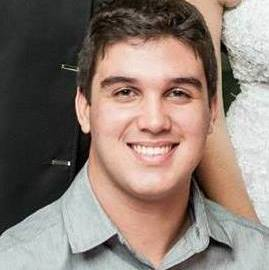
\includegraphics[width=1.5in,clip,keepaspectratio]{antunes.jpg}}
\noindent {\bf Antunes Dantas da Silva}  Nasceu em Picuí, interior do estado brasileiro Paraíba. Possui formação técnica em Manutenção e Suporte em Informática pelo Instituto Federal da Paraíba Campus Campina Grande. Foi membro do Grupo de Pesquisa em Redes Convergentes. Atualmente, está na graduação em Ciência da Computação, pela Universidade Federal de Campina Grande. É membro do Programa de Educação Tutorial, onde desenvolve o Sistema de Avaliação Docente, orientado pelo professor doutor Matheus Gaudêncio do Rêgo. Tem interesse em Engenharia de \textit{Software}, Desenvolvimento de Sistemas e Telecomunicações.  

\vspace{1.0cm}
\parpic{
\includegraphics[width=1.5in,clip,keepaspectratio]{gabriel.jpg}}
\noindent {\bf Gabriel Silva Vinha} nasceu no Brasil, no estado de São Paulo e na cidade de São Paulo. Foi selecionado, no ano de 2014, pela embaixada dos Estados Unidos da América como um dos representantes da juventude pelo programa Jovens Embaixadores. Participou do programa de monitoria no Departamento de Sistemas e Computação, na Universidade Federal de Campina Grande. Atualmente, está na graduação em ciência da computação, pela Universidade Federal de Campina Grande. É membro do Laboratório de Sitemas Distribuídos e do \textit{Software Practices Laboratory}. É desenvolvedor part-time em um projeto da parceria entre o Laboratório de Sitemas Distribuídos, \textit{Software Practices Laboratory}, Lenovo Brasil e \textit{RedHat International}. Tem interesse na área de desenvolvimento web, com foco em aplicações e sistemas em nuvem.

\vspace{1.0cm}
\parpic{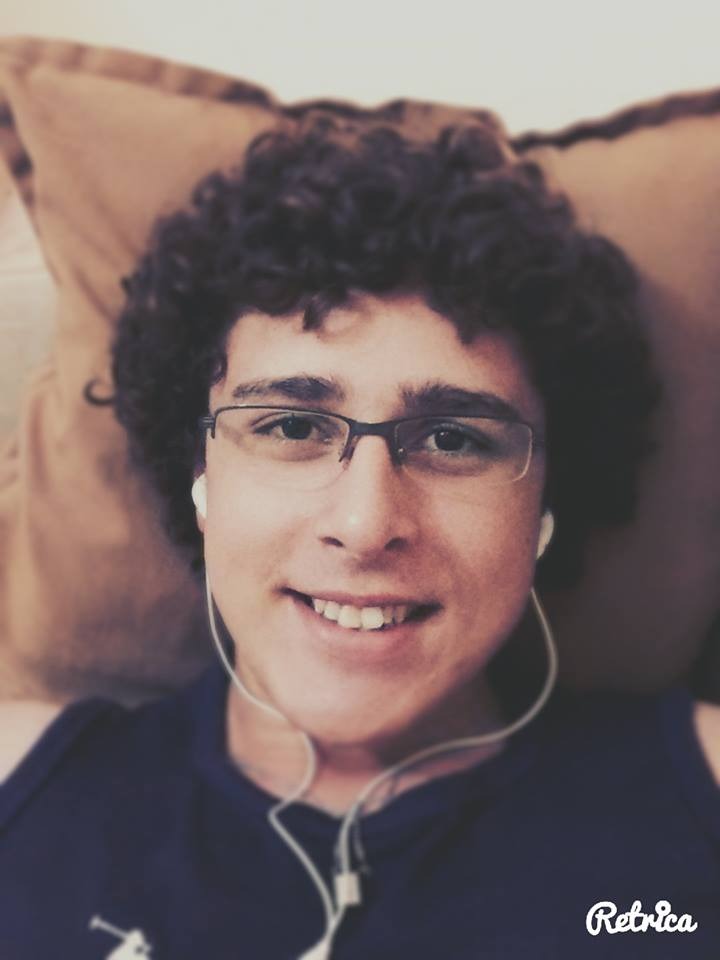
\includegraphics[width=1.5in,clip,keepaspectratio]{italo.jpg}}
\noindent {\bf Italo Menezes de L. Poroca} nasceu em Recife, capital de Pernambuco, Brasil. Graduando do curso de Ciência da Computação pela Universidade Federal de Campina Grande, participou do Programa de Iniciação Científica Jr. pela OBMEP em parceria com o IMPA e o CNPq. Fez curso técnico em Desenvolvimento para \textit{Web}. Atualmente, é membro do projeto de capacitação da Sony do Laboratório de Sistemas Embarcados e Computação Pervasiva (\textit{Embedded Lab}). Tem interesse em Engenharia de \textit{Software}e Desenvolvimento para Sistemas Embarcados, com foco em \textit{mobile} e \textit{web}.

\vspace{1.0cm}
\parpic{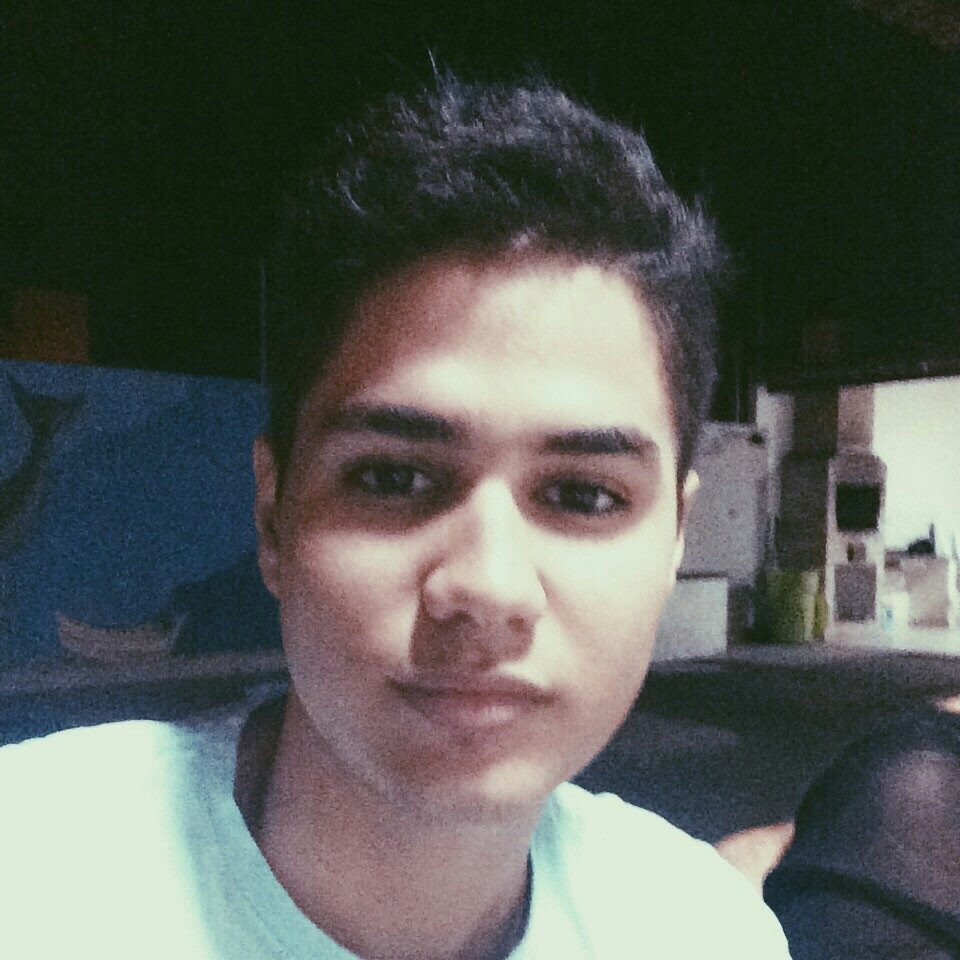
\includegraphics[width=1.5in,clip,keepaspectratio]{valter.jpg}}
\noindent {\bf Valter Vinícius Marinho de Lucena} Nasceu em Patos, Paraíba, Brasil. Possui formação técnica em Manutenção e Suporte em Informática pelo Instituto Federal da Paraíba - Campus Patos. Atualmente graduando em Ciência da Computação pela Universidade Federal de Campina Grande.


%\end{tabular}
%\end{table}

%--------------------------------------------------------------------------------------------------
% FIM DO ARTIGO
%--------------------------------------------------------------------------------------------------
\end{document}
